\section{Architecture}\label{s:arch}


\begin{figure}[ht]
	\centering
	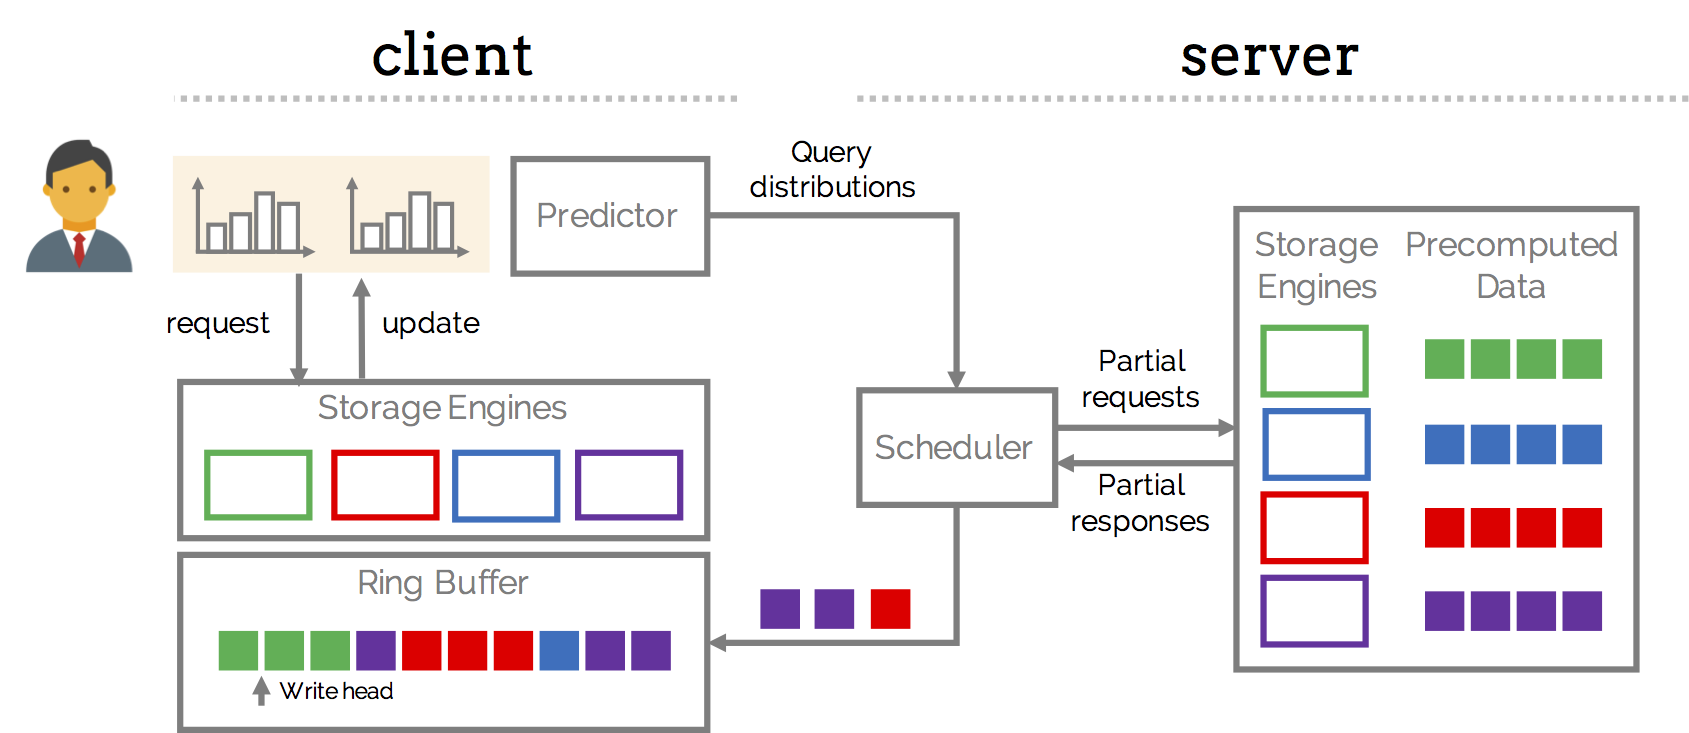
\includegraphics[width=1\columnwidth]{figures/arch}
 	\caption{System Architecture}
  \label{fig:arch}
\end{figure}

\ewu{copied from assignment readme}
Figure~\ref{fig:arch} represents the overall architecture of the system and will be used to introduce the major files.
From left to write, the developer creates visualization charts as wrappers around query templates. When the viz are instantiated, the query templates are registered with the server, so the server can instantiate the appropriate precomputed data structures. The query templates basically parameterize SQL queries.

When a user interacts with the viz (in this case, by hovering over bars), it generates parameter values for the visualization's corresponding query template. The combination is called a query, which is registered with the client Engine. If the data to answer the query is already in the client's cache, then the appropriate client data structure will compute the result and trigger a call back to update the appropriate visualizations.

If data is not available, then the requester will turn the request into a query distribution (where the query has probability 1, and everything else has probability 0) and sends the distribution to the server. The requester's other job is to continuously predict the future query distribution and send it to the server. The impulse distribution is only used when the user actually runs a query that is not in the cache.

The server's manager is basically an infinite loop that can continuously send data to the client. The instantiated data structures read from pre-computed cache files to answer queries in the current query distribution and sends a byte stream to the client.

The client recieves and caches the byte stream into a simple ring buffer. Everytime it detects a usable block of bytes, it sends it to the appropriate data structure to decode and use to answer client queries.


Data structures represent different typs of storage engines that could answer user queries. Data structure objects are represented as triangles in the architecture, they read cached files generated ahead of time (offline). They are the workhorse for answering queries.

There are a few key concepts that are important to understand how they work.

\begin{enumerate}
\item Data structures are instantiated with a query template (e.g., SELECT * WHERE a = ? AND b = ? ...) and precomputes all possible assignments to those parameters.
\item For a given data structure, it's query input is the ID of the query template and the values for the parameters.
\item Data structures send a block of byte-encoded data to the client, which needs to decode the bytes.
\item On the client, once the bytes are (optionally) decoded into javascript objects, the data structure still needs to know which queries the data can answer. To do so, we basically hash the parameter values and use it as a lookup key.
\item All of this means that we need to carefully ensure that data and queries are represented in exactly the same way in the client, the web server, and the offline scripts.
\end{enumerate}
